\documentclass[12pt,letterpaper,onecolumn]{article} % Declara tipo de documento
%% Declara paquetes usados en el documento
\usepackage{amsfonts,amsmath,amssymb,amsthm,dsfont} % Escribir símbolos matemáticos
\usepackage[utf8]{inputenc} % Incluir acentos en UTF-8
\usepackage{graphicx} % Incluir figuras
\usepackage{subcaption} % Escribe pies en subfiguras
\usepackage{parskip} % Incluir saltos de líneas entre párrafos (mismo efecto que \\)
\usepackage[nottoc]{tocbibind} % Agrega sección de referencias a la tabla de contenido
\usepackage{fancyhdr,lastpage} % Encabezados y pies de página

\setlength{\parindent}{20pt} % Aumenta la sangría al inicio del párrafo
%% Declara estilo de encabezados y pies de páginas
\pagestyle{fancy}
\fancyhf{}
\lhead{\footnotesize{Numerical Estimation of Rodenticide Dispersal}} % lado izquierdo del encabezado de página
\rhead{\footnotesize{GECI}} % lado derecho del encabezado de página
\rfoot{\scriptsize{\thepage\ de \pageref{LastPage}}} % pie de página
%% Encabezado del artículo
\title{Improving the efficiency of aerial rodent eradications: The \textit{ad hoc} development of NERD, an original mathematically founded implementation}
\author{Evaristo Rojas-Mayoral, Federico A. M\'endez-S\'anchez, \\
Araceli Samaniego-Herrera, Ana G. C\'ardenas-Tapia, \\
Braulio Rojas-Mayoral, Alfonso Aguirre-Mu\~noz}
%% Inicia documento con encabezado e índice
\begin{document}
\maketitle
\tableofcontents
\clearpage
%% Llama secciones del documento que se encuentran en archivos TEX separados
\section{Abstract}

Invasive rodents are present on approximately 90\% of the world’s islands and constitute one of the most serious threats to both endemic and native island species. The eradication of rodents is central to island conservation efforts and the aerial broadcast of rodenticide bait is the preferred dispersal method. To maximize the efficiency of rodent eradication campaigns utilizing aerial dispersal methods, the generation of accurate and real-time bait density maps are needed. Traditionally, creating maps to estimate the spatial dispersion of bait on the ground has been carried out using GIS, which is based on several untested assumptions and is time intensive. To improve accuracy and speed up the evaluation of aerial operations, we developed a new tool called NERD: Numerical Estimation of Rodenticide Dispersal. NERD is the implementation of a mathematical model, in the computing language of MATLAB, which performs calculations with increased accuracy, displaying results almost in real-time. At its core, the model is a probability density function describing bait density as a function of the aperture diameter of the bait bucket, the helicopter speed, and the wind speed. NERD also facilitates the planning of helicopter flight paths and allows for the instant identification of bait gaps. NERD was effectively used in two recent and successful rodent eradication campaigns in Mexico: the mouse eradication on San Benito Oeste Island (400 ha) in the Mexican Pacific, and the rat eradication on Cayo Centro Island (539 ha) from Banco Chinchorro, in the Mexican Caribbean. The latter represents the largest rodent eradication on a wet tropical island to date. NERD has proven its efficacy and and can significantly reduce the overall cost of large-scale rodent eradication campaigns.

\section{Introduction}
The effects of invasive rodent species on island ecosystems are incredibly deleterious, especially on islands that present high levels of endemism and islands that have evolved in the absence of predators occupying similar niches to the invasive rodent species or higher order predators \cite{Meyers2000}. Under these circumstances, the presence of invasive rodents on islands can lead to the rapid decline and extinction of native plant and animal species (\cite{Medina2011} and \cite{Towns2006}). The resultant losses are reflected in reduced biodiversity on the affected islands and in many cases, the emergence of the invasive rodent as the dominant species. In severe cases of rodent invasion, key island ecosystem services are lost (e.g. \cite{Towns2006}). As such, the first step in island restoration and biodiversity recovery is the eradication of invasive rodent species.

Of the various means of rodent eradication on islands, the aerial broadcast of rodenticide bait is one of the preferred methods given the obvious advantages. The aerial dispersal of rodenticide can cover large areas quickly and can mitigate the challenges associated with complex topography. To assess the effectiveness of an aerial operation, bait density maps are required to evaluate the spatial variation of bait availability on the ground. However, creating bait density maps has been traditionally slow and impractical in the field, while taking in situ measurements to evaluate aerial work is difficult given the challenges associated with field conditions, topography, and available manpower.

To address these challenges, we have developed NERD: Numerical Estimation of Rodenticide Dispersal. NERD facilitates the planning of helicopter rodenticide dispersal campaigns by generating bait density maps automatically and allowing for the instant identification of bait gaps with fewer in situ measurements. NERD consists of two components, a mathematical model and its implementation in the computing language of MATLAB. The mathematical model is based on prior calibration experiments in which the mass flow of rodenticide through a bait bucket is measured. At its core, the model is a probability density function that describes bait density as a function of bucket aperture diameter, helicopter speed, and wind speed.

\section{Formulation}
The objective of this section is to show that the function $\sigma(x,y)$ used to represent the superficial bait density (kg/m$^2$), must comply with the following property
$$\int_{-\frac{w}{2}}^{+\frac{w}{2}} \sigma(x)dx=\frac{\dot{m}}{s},$$
where $\dot{m}$ is the bait flow (kg/s), $s$ is the speed of the helicopter (m/s), and $w$ is the swath width (m).

% Ambiente para incluir figura centrado, con pies de figuras y etiqueta para usar como referencia cruzada
\begin{figure}[h]
  \centering
  \includegraphics[width=120mm]{../resultados/png/helicopter-flight-path.png}
  \caption{Schematic of a helicopter’s flight path over a swath with three
  dispersal cells; $w$ is the swath width; $\delta y$ is the distance between two
  GPS points; and $A_{\mbox{cell}}$ is the area of a dispersal cell.}
  \label{fig:esquemaHelicoptero}
\end{figure}

We set the origin of a Cartesian coordinate system on the middle point of the
inferior side of a rectangle with base $w$ and height $\delta y$. This way, the
inferior side is found at $y=0$, the superior side at $y=\delta y$,the left side
at $x=-\frac{w}{2}$ and the right side at $x=+\frac{w}{2}$.

After the helicopter completes a pass, in each point $(x,y)$ of the rectangle a superficial bait density is obtained $\sigma(x,y)$. The definition of the superficial bait density of mass $m$ indicates that $\sigma(x,y)=\frac{dm}{dA}$. Rewriting the superficial density substituting $dA$ by $dydx$ and integrating along the dispersion cell, it follows that
% Ambiente para incluir ecuación y etiquetarla
\begin{equation}
  \delta m=\int_{-\frac{w}{2}}^{+\frac{w}{2}} \int_{0}^{\delta y} \sigma(x,y)dydx.
  \label{eq:masaEsIntegralDobleDeDensidad}
\end{equation}

\begin{figure}
  \centering
  % Ambiente para incluir subfigura
  \begin{subfigure}[b]{0.45\textwidth}
    
\includegraphics[width=\textwidth]{../resultados/png/constant-bait-density.png}
    \caption{Constant bait density along each swath.}
    \label{fig:densidadConstante}
  \end{subfigure}
  \begin{subfigure}[b]{0.45\textwidth}
    
\includegraphics[width=\textwidth]{../resultados/png/variable-bait-density.png}
    \caption{Variable bait density along each swath.}
    \label{fig:densidadVariable}
  \end{subfigure}
  \caption{
  Hypothetical island with bait swaths. Each green band represents one bait swath. The intensity of the bait swath color corresponds to its density, with darker colors indicating greater densities.
  }
\end{figure}


Assuming superficial density is uniform with respect to the helicopter’s flight
path, represented in Figure \ref{fig:densidadConstante}, equation \eqref{eq:masaEsIntegralDobleDeDensidad} becomes
\begin{equation}
  \frac{\delta m}{\delta y}=\int_{-\frac{w}{2}}^{+\frac{w}{2}}\sigma(x)dx.
  \label{eq:densidadLineal}
\end{equation}

The left-hand side of the equation represents the linear bait density which is
related with the mass flow of bait from the bucket and the speed of the
helicopter.  A helicopter equipped with a dispersion bucket with a constant mass
flow rate,
\begin{equation}
  \dot{m}=\frac{\delta m}{\delta t}
  \label{eq:flujoMasico}
\end{equation}
flies from the point $(0,0)$ to the point $(0,\delta y)$ with a speed of
\begin{equation}
  s=\frac{\delta y}{\delta t}.
  \label{eq:rapidez}
\end{equation}

Combining equations \eqref{eq:flujoMasico} and \eqref{eq:rapidez}, the linear bait
density
\begin{equation}
  \frac{\delta m}{\delta y}=\frac{\dot{m}}{s},
  \label{eq:densidadLinealEsflujoSobreRapidez}
\end{equation}
is obtained.

Finally, setting equations \eqref{eq:densidadLineal} and \eqref{eq:densidadLinealEsflujoSobreRapidez} equal to each other, we obtain
\begin{equation}
  \int_{-\frac{w}{2}}^{+\frac{w}{2}} \sigma(x)dx=\frac{\dot{m}}{s}.
  \label{eq:integralDeDensidadEsflujoSobreRapidez}
\end{equation}

Equation \eqref{eq:integralDeDensidadEsflujoSobreRapidez}  relates a density that is needed in the field with the variables of the bait dispersal mechanism.

\section{Calibration}
Assuming the density is independent of $x$, i.e. $\sigma$ does not change along the swath width, equation \eqref{eq:integralDeDensidadEsflujoSobreRapidez} can be easily solved to obtain

\begin{equation}
  \sigma = \frac{\dot{m}}{s\cdot w}.
  \label{eq:densidadEsFlujoSobreProductoRapidezPorAncho}
\end{equation}

In order to write equation \eqref{eq:densidadEsFlujoSobreProductoRapidezPorAncho} as a function of the aperture diameter of the bait bucket, we express the mass flow rate of bait as a function of the aperture diameter, $\dot{m}(d)$. To do this, the bait in the bucket was weighed and the time required to empty the bucket was measured and repeated using several aperture diameters. Figure \ref{fig:flujoDeApertura} shows the results from the calibration as well as the fitted model.

\begin{figure}
  % Generada por plotFlow.m
  \centering
  \begin{subfigure}[b]{0.45\textwidth}
    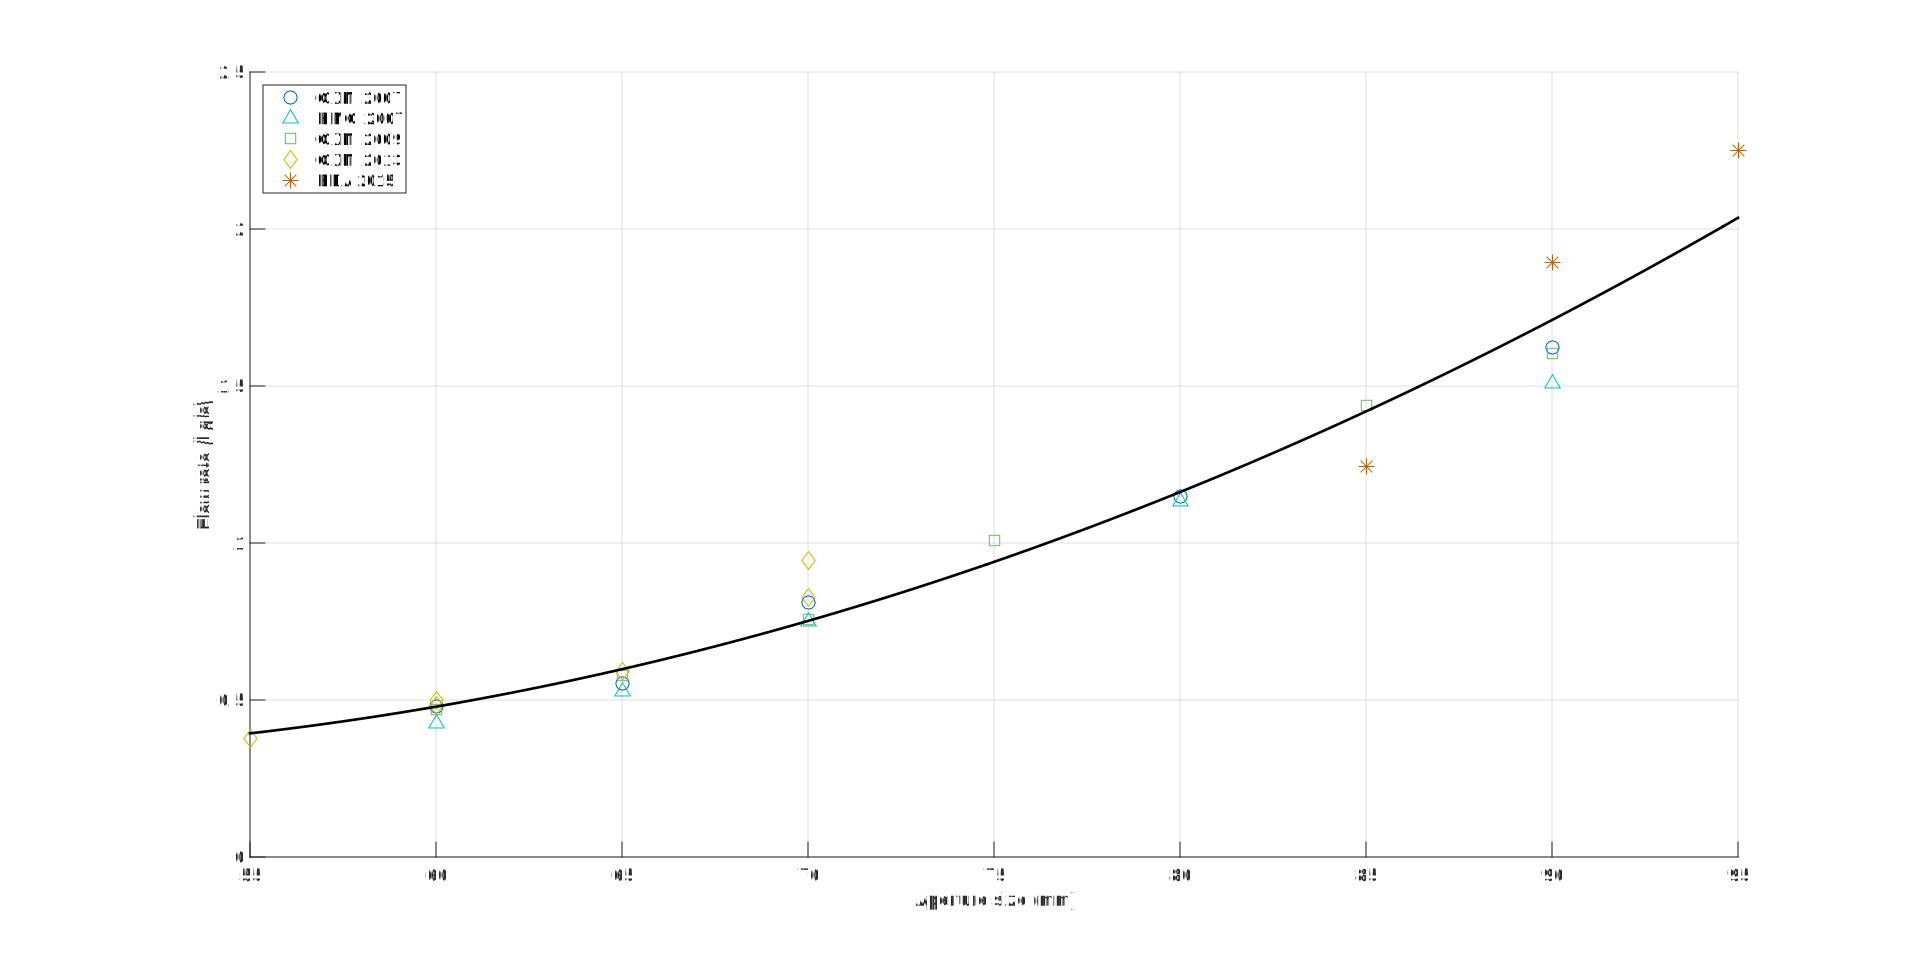
\includegraphics[width=\textwidth]{../resultados/png/flujo-de-apertura.png}
    \caption{$\dot{m}(d)$}
    \label{fig:flujoDeApertura}
  \end{subfigure}
  \begin{subfigure}[b]{0.45\textwidth}
    % Aquí­ va la figura generada a partir `images\density.svg`.
    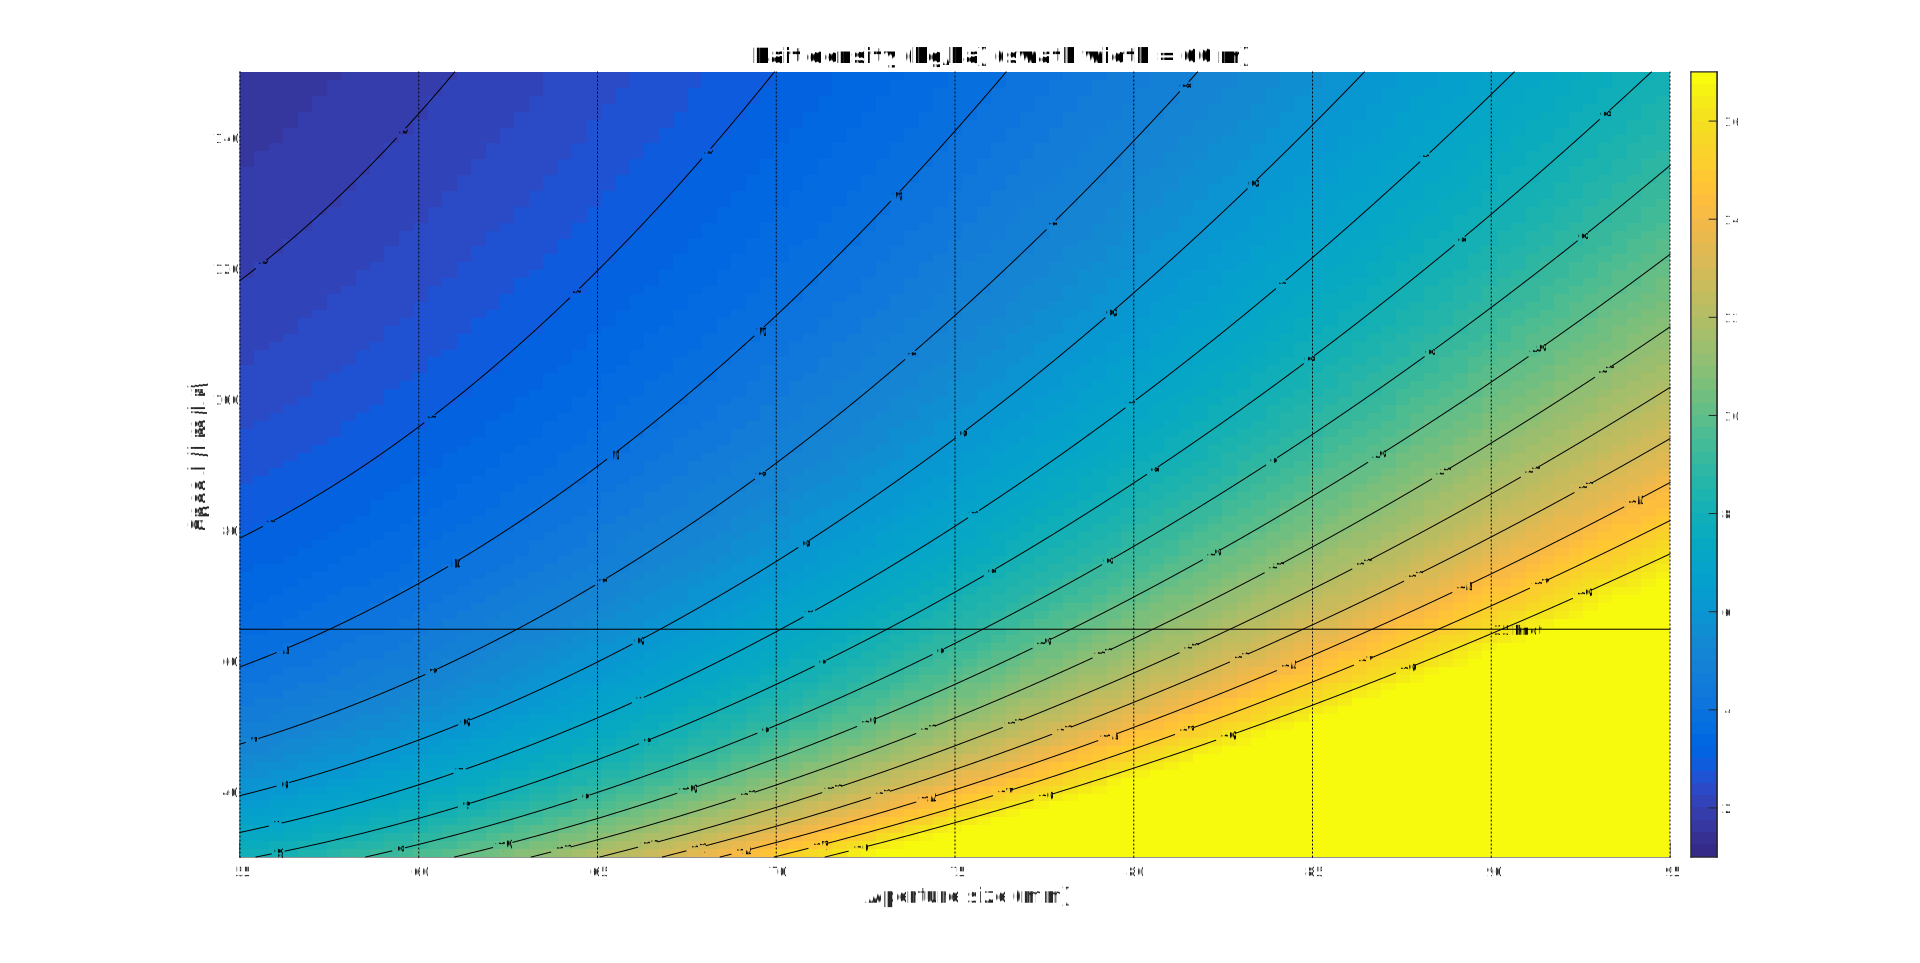
\includegraphics[width=\textwidth]{../resultados/png/densidad-de-apertura-y-rapidez.png}
    \caption{$\sigma(d,s)= \frac{\dot{m}(d)}{s\cdot w}$}
    \label{fig:densidadDeAperturaYRapidez}
  \end{subfigure}
  \caption{ \ref{fig:flujoDeApertura}
  Flow rate $\dot{m}$ (kg/s) as a function of aperture diameter, $d$
  (mm); each symbol represents a calibration event and the black curve is the
  quadratic model fitted to the data. \ref{fig:densidadDeAperturaYRapidez}
  Surface bait density $\sigma$ (kg/ha) as a function of aperture diameter $d$
  (mm), and speed $s$ (km/hr). The horizontal axis shows the aperture diameter of
  the bait bucket and the vertical axis shows the helicopter's speed. The
  resulting bait density on the ground is shown in the second vertical color axis.}
\end{figure}

The resulting three-dimensional model, $$\sigma(d,s)= \frac{\dot{m}(d)}{s\cdot w},$$ is shown in Figure \ref{fig:densidadDeAperturaYRapidez}. During the planning stage of an eradication campaign, this model can be used to determine the diameter of the bait bucket needed to achieve the desired bait density on the ground, ensuring efficient bait coverage, while maximizing resources, time and manpower.

\section{Application}
For a given island, a particular bait density is required on the ground for a successful rodent eradication. This density is determined after studying the ecosystems of the island and the biology of the invasive target species. Given the required bait density and the total area of the island, the minimum amount of bait needed for the eradication operation can be calculated using NERD. While planning helicopter flights paths, it is assumed that the bait density within each swath is constant, but variable between swaths.

Assuming a variable bait density along each swath but uniform density across the
swath, we can estimate bait density with greater precision after the aerial
dispersal given that the bait density for each cell is calculated between two consecutive points recorded by the GPS. This case considers the effects on
density when the helicopter flies with variable speed (Figure \ref{fig:densidadSimetrica}).

To account for the well known fact that we have a higher density of rodenticide right bellow of the helicopter and lower densities along the edges of the swath, we can assume a variable bait density both along and across each swath.  This allows for the detection of areas where the bait density is below the lower limit of the target bait density or of gaps on the ground without any bait (Figure \ref{fig:densidadSimetrica}).

\begin{figure}
  \centering
  \begin{subfigure}[b]{0.45\textwidth}
    \includegraphics[width=\textwidth]{../resultados/png/symmetric-bait-density.png}
    \caption{
    Symmetric bait density
    }
    \label{fig:densidadSimetrica}
  \end{subfigure}
  \begin{subfigure}[b]{0.45\textwidth}
    
\includegraphics[width=\textwidth]{../resultados/png/asymmetric-bait-density.png}
    \caption{
    Asymmetric bait density
    }
    \label{fig:densidadAsimetrica}
  \end{subfigure}
  \caption{
  \ref{fig:densidadSimetrica}
  Hypothetical island with symmetric variable bait density across each swath.
  \ref{fig:densidadAsimetrica}
  Hypothetical island with asymmetric variable bait density across each swath.}
\end{figure}

To account for the effect of the wind on the bait density profile, an asymmetric
and fully variable bait density distribution within each swath is allowed
(Figure \ref{fig:densidadAsimetrica}).

\section{Discussion}
NERD: Numerical Estimation of Rodenticide Dispersal provides provides a mathematical model, based on past calibration experiments in which the mass flow of bait through a bait bucket is measured, that describes bait density as a function of the aperture diameter, the helicopter speed, and the wind speed. NERD can assist in the planning of the aerial operations as well as during the eradication, giving near real-time feedback allowing for on-the-spot corrections during the operation. The final product of NERD is a bait density map generated in a matter of seconds, which permits better planning and the automatization of an otherwise difficult and slow processes, while allowing for the instant identification of bait gaps and the efficient use of resources.

%% Genera seción de referencias
\bibliographystyle{unsrt}
\bibliography{references}
\end{document}
